\documentclass{beamer}

\usepackage{times}

\usepackage{verbatim}
\usepackage{color}
\usepackage{listings}

\usepackage[german]{babel}
\usepackage[latin1]{inputenc}

\usepackage{multicol}

\usepackage{beamerthemesplit}
\usetheme{Malmoe}

%\usepackage{pgfpages}
%\pgfpagesuselayout{resize to}[a4paper,landscape]

\definecolor{lbcolor}{rgb}{0.92,0.92,0.92}
\definecolor{cmtcolor}{rgb}{0.0,0.5,0.0}
\lstset{numbers=left,
        numberstyle=\tiny,
        keywordstyle=\color{blue}\bfseries\sffamily,
        identifierstyle=\ttfamily,
        commentstyle=\em,
        stringstyle=\ttfamily,
        extendedchars=true,
        showstringspaces=false,
        language=c++,
        backgroundcolor=\color{lbcolor},
        commentstyle=\color{cmtcolor}}

\title{HF-ICT Informatik Vorkurs}
\author{David Herzig (dave.herzig@gmail.com)}
\date{\today}

\begin{document}

\frame{\titlepage}

\setcounter{tocdepth}{1}

\frame
{
	\frametitle{Inhalt}
	\begin{itemize}
	\item Theoretical, Practical, Technological, ...
	\item Grundlagen Informatik (Zahlensysteme, Gr"ossen, ...)
	\item Einf"uhrung C++
	\item Vorbereitung Aufnahmepr"ufung
	\end{itemize}
}

\frame
{
	\frametitle{Inhalt}
	Unterlagen
	\begin{itemize}
	\item Unterricht: Folien und Aufgaben
	\item Buch: C++ f"ur Spieleprogrammierer, (ISBN 13: 978-3446421400)
	\item Internet: http://www.mingw.org (C++ Compiler)
	\item Editor: http://notepad-plus-plus.org/
	\end{itemize}
}

\frame
{
	\frametitle{Inhalt}
	Aufgaben / "Ubungen
	\begin{itemize}
	\item "Ubungen sind sehr wichtig !!!
	\item "Ubungen w"ahrend dem Unterricht
	\item Pro Woche ein Aufgabenblatt
	\item Aktive Teilnahme bei Besprechung der "Ubungen ist erw"unscht
	\end{itemize}
}

\section{Grundlagen Informatik}
\frame
{
	\frametitle{Grundlagen Informatik}
	\begin{itemize}
	\item Zahlensysteme
	\item Gr"ossen der Informatik
	\item ASCII Code
	\item Logik
	\item Aufbau eines Computers
	\end{itemize}
}

\frame
{
	\frametitle{Zahlensysteme}
	{\small Bei dem Begriff Zahlensystem handelt es sich um ein Verfahren zur Darstellung von Zahlen,
	das auf einer mathematischen Basis aufbaut. Dabei handelt es sich in der Regel um eine
	nat"urliche Zahl mit der Eigenschaft gr"osser oder gleich 2. Eine Zahl wird durch
	Aneinanderreihung der einzelnen Ziffernzeichen gebildet, wobei die Anzahl der verschiedenen
	Ziffernzeichen mit der Basis identisch ist. Beim Dezimalsystem, einem Zahlensystem mit der
	Basis 10 gibt es demnach 10 Ziffernzeichen.}
	
	\begin{itemize}
	\item Umwandlung vom Dezimalsystem
	\item Umwandlung ins Dezimalsystem
	\item Umwandlung Bin"ar - Hexadezimal
	\end{itemize}
}

\frame
{
	\frametitle{Zahlensysteme - Tabelle}
	{\tiny
	\begin{tabular}{c|c|c|c}
	Dezimalsystem & Bin"arsystem & Oktalsystem & Hexadezimalsystem \\
	\hline
	0 & 0 & 0 & 0 \\
	1 & 1 & 1 & 1 \\
	2 & 10 & 2 & 2 \\
	3 & 11 & 3 & 3 \\
	4 & 100 & 4 & 4 \\
	5 & 101 & 5 & 5 \\
	6 & 110 & 6 & 6 \\
	7 & 111 & 7 & 7 \\
	8 & 1000 & 10 & 8 \\
	9 & 1001 & 11 & 9 \\
	10 & 1010 & 12 & A \\
	11 & 1011 & 13 & B \\
	12 & 1100 & 14 & C \\
	13 & 1101 & 15 & D \\
	14 & 1110 & 16 & E \\
	15 & 1111 & 17 & F \\
	16 & 10000 & 20 & 10 \\
	17 & 10001 & 21 & 11 \\
	\end{tabular}
	}
}

\frame
{
	\frametitle{Zahlensysteme - Umwandlung vom Dezimalsystem}
	Umwandlung einer Zahl x vom Dezimalsystem in ein System mit Basis b.\\
	\vspace{3mm}
	\begin{displaymath}
	\begin{array}{ll}
	x : b = a_0 \quad REST \quad b_0 \\
	a_0 : b = a_1 \quad REST \quad b_1 \\
	a_1 : b = a_2 \quad REST \quad b_2 \\
	\vdots \\
	a_{n-1} : b = 0 \quad REST \quad b_n
	\end{array}
	\end{displaymath}
	\vspace{3mm}
	L"osung: $b_n \dots b_2 b_1 b_0$	
}

\frame
{
	\frametitle{Zahlensysteme - Beispiel}
	$101_{10} \Rightarrow ?_2$\\
	\vspace{3mm}
	\begin{displaymath}
	\begin{array}{ll}
	101 : 2 = 50 \quad REST \quad 1 \\
	50 : 2 = 25 \quad REST \quad 0 \\
	25 : 2 = 12 \quad REST \quad 1 \\
	12 : 2 = 6 \quad REST \quad 0 \\
	6: 2 = 3 \quad REST \quad 0 \\
	3 : 2 = 1 \quad REST \quad 1 \\
	1 : 2 = 0 \quad REST \quad 1
	\end{array}
	\end{displaymath}
	\vspace{3mm}
	L"osung: $1100101$
}

\frame
{
	\frametitle{"Ubungen}
	\begin{enumerate}
	\item $53_{10} \Rightarrow ?_2$
	\item $1023_{10} \Rightarrow ?_{16}$
	\item $452_{10} \Rightarrow ?_8$
	\item $66_{10} \Rightarrow ?_2$
	\end{enumerate}
}

\frame
{
	\frametitle{"Ubungen - L"osungen}
	\begin{enumerate}
	\item $53_{10} \Rightarrow 110101_2$
	\item $1025_{10} \Rightarrow 3FF_{16}$
	\item $452_{10} \Rightarrow 704_8$
	\item $66_{10} \Rightarrow 1000010_2$
	\end{enumerate}
}

\frame
{
	\frametitle{Zahlensysteme - Umwandlung ins Dezimalsystem}
	Umwandlung einer Zahl x im System mit Basis b in eine Dezimalzahl.\\
	Beispiel Zahl x: $\underbrace{1}_\text{Ziffer 3} \underbrace{2}_\text{Ziffer 2} \underbrace{3}_\text{Ziffer 1} \underbrace{4}_\text{Ziffer 0}$\\
	\vspace{3mm}
	\begin{displaymath}
	\begin{array}{ll}
	Dezimalzahl = \\
	Ziffer \, n \cdot (b)^n \\
	+ \dots \\
	+ Ziffer \, 2 \cdot (b)^2 \\
	+ Ziffer \, 1 \cdot (b)^1 \\
	+ Ziffer \, 0 \cdot (b)^0
	\end{array}
	\end{displaymath}
}

\frame
{
	\frametitle{Zahlensysteme - Beispiel}
	$1101110_{2} \Rightarrow ?_{10}$\\
	\vspace{3mm}
	$\overbrace{1}^\text{6} \overbrace{1}^\text{5} \overbrace{0}^\text{4} \overbrace{1}^\text{3} \overbrace{1}^\text{2} \overbrace{1}^\text{1} \overbrace{0}^\text{0}$
	\vspace{3mm}
	\begin{displaymath}
	1 \cdot 2^6 + 1 \cdot 2^5 + 0 \cdot 2^4 + 1 \cdot 2^3 + 1 \cdot 2^2 + 1 \cdot 2^1 + 0 \cdot 2^0 = 110
	\end{displaymath}
	\vspace{3mm}
	L"osung: $110$
}

\frame
{
	\frametitle{Zahlensysteme - Beispiel}
	$F5A_{16} \Rightarrow ?_{10}$\\
	\vspace{3mm}
	$\overbrace{F}^\text{2} \overbrace{5}^\text{1} \overbrace{A}^\text{0}$
	\vspace{3mm}
	\begin{displaymath}
	15 \cdot 16^2 + 5 \cdot 16^1 + 10 \cdot 16^0 = 3930
	\end{displaymath}
	\vspace{3mm}
	L"osung: $3930$
}

\frame
{
	\frametitle{"Ubungen}
	\begin{enumerate}
	\item $101110_{2} \Rightarrow ?_{10}$
	\item $712_{8} \Rightarrow ?_{10}$
	\item $AF5_{16} \Rightarrow ?_{10}$
	\item $111000_{2} \Rightarrow ?_{10}$
	\end{enumerate}
}

\frame
{
	\frametitle{"Ubungen - L"osungen}
	\begin{enumerate}
	\item $101110_{2} \Rightarrow ?46_{10}$
	\item $712_{8} \Rightarrow 458_{10}$
	\item $AF5_{16} \Rightarrow 2805_{10}$
	\item $111000_{2} \Rightarrow 56_{10}$
	\end{enumerate}
}

\frame
{
	\frametitle{Zahlensysteme - Umwandlung Bin"ar - Hexadezimal}
	Direkte Umwandlung zwischen dem Bin"arsystem und dem Hexadezimalsystem.\\
	Bei dieser Methode werden die Ziffern von rechts her in Gruppen mit
	je 4 Ziffern aufgeteilt.\\
	{\small
	$1111001001101 \Rightarrow$ Einteilung in Gruppen $\Rightarrow 1 \quad 1110 \quad 0100 \quad 1101$
	}\\
	\vspace{3mm}
	Nun wird jede Gruppe umgerechnet:\\
	\vspace{3mm}
	$\underbrace{1}_\text{1} \quad \underbrace{1110}_\text{E} \quad \underbrace{0100}_\text{4} \quad \underbrace{1101}_\text{D}$\\
	\vspace{3mm}
	Funktioniert auch in anderer Richtung, indem aus jeder hexadezimalen Ziffer vier bin"are Ziffern erstellt werden.
}

\frame
{
	\frametitle{"Ubungen}
	\begin{enumerate}
	\item $101110_{2} \Rightarrow ?_{16}$
	\item $111011101110_{2} \Rightarrow ?_{16}$
	\item $ABFD82_{16} \Rightarrow ?_{2}$
	\item $12345_{16} \Rightarrow ?_{2}$
	\end{enumerate}
}

\frame
{
	\frametitle{"Ubungen - L"osungen}
	\begin{enumerate}
	\item $101110_{2} \Rightarrow 2E_{16}$
	\item $111011101110_{2} \Rightarrow EEE_{16}$
	\item $ABFD82_{16} \Rightarrow 101010111111110110000010_{2}$
	\item $12345_{16} \Rightarrow 10010001101000101_{2}$
	\end{enumerate}
}

\frame
{
	\frametitle{Zahlensysteme - "Ubungstool}
	"Ubungstool zur Umwandlung von Zahlen in verschiedenen Zahlensystemen. Steht auf dem OLAT System zur Verf"ugung.\\
	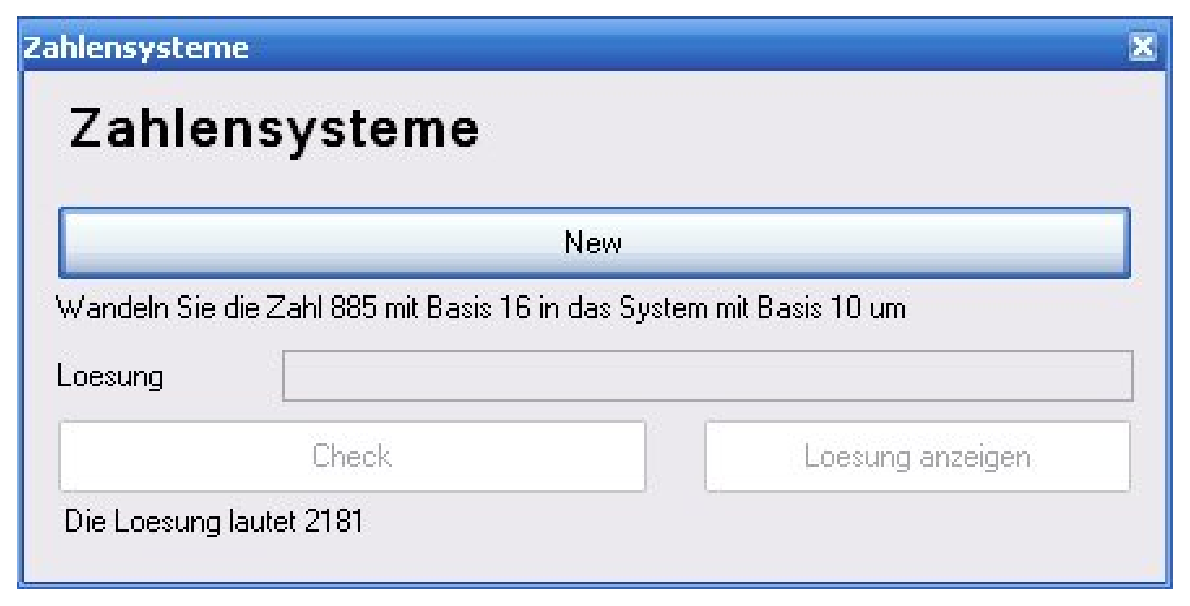
\includegraphics[width=150pt]{zahlensysteme.ps}
}

\frame
{
	\frametitle{L"osung Aufgabenblatt 1}
	Aufgabe 1
	\begin{enumerate}
	\item $1010110111_{2} = 695_{10}$
	\item $25_{16} = 100101_{2}$
	\item $2345_{8} = 1253_{10}$
	\item $ABCD_{16} = 1010101111001101_{2}$
	\item $1046_{10} = 416_{16}$
	\end{enumerate}
}

\frame
{
	\frametitle{L"osung Aufgabenblatt 1}
	Aufgabe 2
	\begin{enumerate}
	\item $12_{10} + ABC_{16} + 1001_{2} = 2769_{10}$
	\item $10011101_{2} + 123_{10} = 118_{16}$
	\item $11_{2} + 77_{8} + FF_{16} = 321_{10}$
	\end{enumerate}
}
\frame
{
	\frametitle{L"osung Aufgabenblatt 1}
	{\tiny
	Aufgabe 3
	\begin{enumerate}
	\item Wieviele Zahlensysteme gibt es?\\
	\emph{Unendlich viele}
	\item Durch was kann ein Zahlensystem charakterisiert werden?\\
	\emph{Basis, zur Verf"ugung stehende Ziffern, Stellenwert}
	\item Wie k"onnte eine direkte Umwandlung vom Bin"arsystem ins Oktalsystem erfolgen?\\
	\emph{Die bin"are Zahl wird in dreier Guppen aufgeteilt.}
	\item Wieviele Stellen werden ben"otigt um eine Zahl Z mit Basis B darzustellen?\\
	$\lfloor log_B(Z) + 1 \rfloor$
	\item "Uberlegen Sie sich, wie man negative Zahlen im Bin"arsystem darstellen k"onnte.\\
	\emph{Es wird ein Bit als Vorzeichen verwendet. Bsp: 1 bedeutet Negativ, 0 bedeutet Positiv.}
	\item Wenn die Menschen mit Ihren Fingern bin"ar z"ahlen w"urden (Finger ausgestreckt = 1, Finger eingezogen = 0), wie hoch k"onnten wir dann z"ahlen?\\
	\emph{Von 0 bis} $2^{10}-1 = 1023$
	\end{enumerate}
	}
}

\frame
{
	\begin{center}
	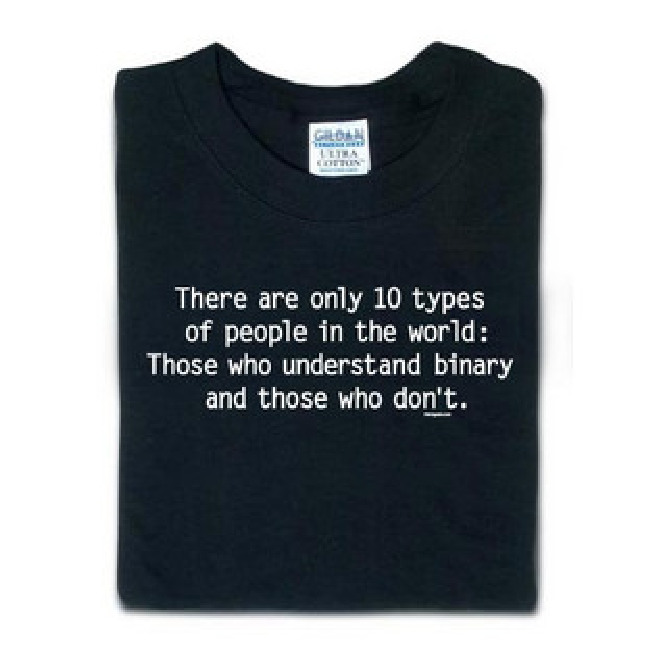
\includegraphics[width=160pt]{binary-people.eps}
	\end{center}
}

\frame
{
	\frametitle{Gr"ossen der Informatik}
	{\small
	\begin{itemize}
	\item Bit (kleinste Einheit: 0 oder 1)
	\item Nibble (4 Bit)
	\item Byte (8 Bit)
	\item 1 kByte ($2^{10}$ Bytes = 1024 Bytes)
	\item 1 MByte (1024 kBytes, 1048576 Bytes)
	\item 1 GByte (Giga)
	\item 1 TByte (Tera)
	\item 1 PByte (Peta)
	\end{itemize}
	Architekturabh"angig (32 Bit, 64 Bit Systeme)
	\begin{itemize}
	\item Halbwort (16 Bit, Architekturabh"angig)
	\item Wort (32 Bit, Architekturabh"angig)
	\item Doppelwort (64 Bit, Architekturabh"angig)
	\end{itemize}
	}
}

\frame
{
	\frametitle{"Ubungen}
	\begin{enumerate}
	\item Was ist die h"ochste Dezimalzahl, welche mit 6 Bits dargestellt werden kann?
	\item Wieviele Bits sind notwendig um die Grossbuchstaben unseres lateinischen Alphabets darzustellen?
	\item Eine Datei der Gr"osse 100 Megabyte soll von einem Computer auf den USB Stick
	"ubertragen werden. Die "Ubertragungsrate betr"agt 480 MBit/s. Wie lange dauert der Kopiervorgang?
	\end{enumerate}
}

\frame
{
	\frametitle{"Ubungen - L"osungen}
	\begin{enumerate}
	\item 6 Bit: $111111_2$ = $63_{10}$
	\item 26 Buchstaben: 5 Bits (32 M"oglichkeiten)
	\item 480 MBit/s = 60 MByte / s. $\frac{100 MByte}{60 MByte/s} = 1.67s$
	\end{enumerate}
}

\frame
{
	\frametitle{ASCII Code}
	Der ASCII Code ist eine 7 Bit Zeichencodierung. Er ordnet bekannten Zeichen
	einen Code zu. Es existieren 128 Zeichen. Um mehr Zeichen codieren zu k"onnen,
	wird heute der Unicode verwendet.\\
	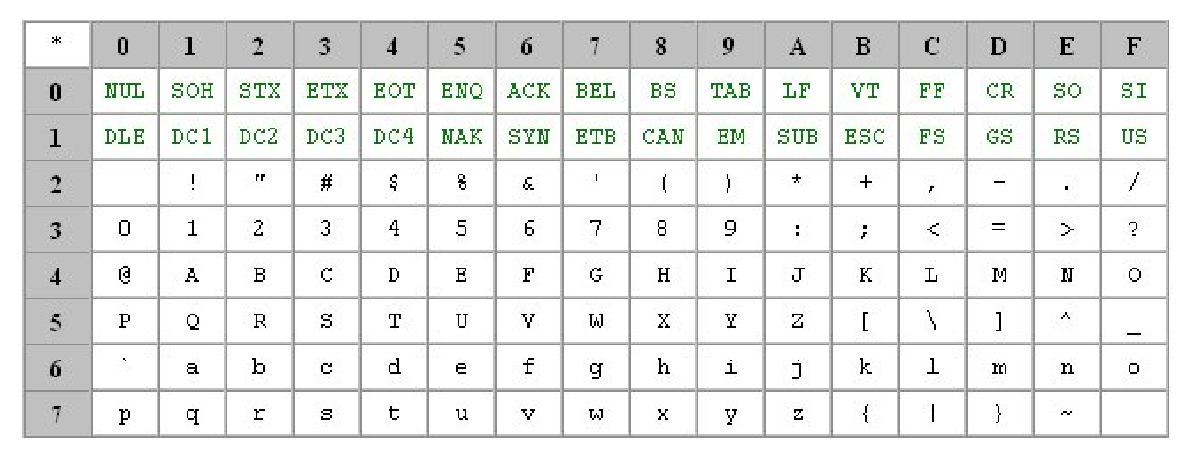
\includegraphics[width=240pt]{ascii.ps}

}

\frame
{
	\frametitle{ASCII Code - Beispiel}
	PULP FICTION\\
	\vspace{3mm}
	Hexadezimal:\\
	50 55 4C 50 20 46 49 43 54 49 4F 4E\\
	\vspace{3mm}
	Dezimal:\\
	80 85 76 80 32 70 73 67 84 73 79 78\\
	\vspace{3mm}
	Bin"ar:\\
	{\tiny 101000 101101 1001100 1010000 100000 100110  1001001 1000011 1010100 1001001 1001111 1001110}\\
}

\frame
{
	\frametitle{"Ubungen}
	\begin{enumerate}
	\item Ein Zeichen hat den Bin"arcode 1111010. Welches Zeichen ist gemeint?
	\item Dekodieren Sie:\\
	{\tiny 010100110100001101001000010101010100110001000101}
	\item Codieren Sie das Wort \emph{Computer} (Hex-Format)
	\end{enumerate}
}

\frame
{
	\frametitle{"Ubungen - L"osungen}
	\begin{enumerate}
	\item Ein Zeichen hat den Bin"arcode 01111010. Welches Zeichen ist gemeint?\\
	z
	\item Dekodieren Sie:\\
	{\tiny 010100110100001101001000010101010100110001000101}\\
	SCHULE
	\item Computer: 43 6F 6D 70 75 74 65 72
	\end{enumerate}
}

\frame
{
	\frametitle{L"osung Aufgabenblatt 2}
	Aufgabe 1
	{\tiny
	\begin{enumerate}

	\item Ein Bildschirm hat eine Aufl"osung von 1024x768 Pixel. Jeder Pixel kann eine
	aus 256 verschiedenen Farben darstellen. Wie viel Speicher wird f"ur die Darstellung
	des ganzen Bildschirms ben"otigt?\\
	Um 256 Farben zu speichern, werden 8 Bits ben"otigt. Das heisst, jeder Pixel hat 1 Byte (1 Byte = 8 Bit).\\
	Der Bildschirm besitzt somit $1024 \cdot 768 \cdot 1 Byte = \underline{768kBytes}$
	
	\item Wieviele Bytes werden ben"otigt, um die hexadezimale Zahl ABCD zu speichern?\\
	Wird man die Zahl ABCD in das bin"are System umgewandelt, so entsteht 1010101111001101.
	Dies sind $\underline{16 Bits = 2 Bytes}$.

	\item Ein Verlag m"ochte gerne ein bestimmtes Buch in elektronischer Form vertreiben.
	Das Buch besitzt im gesamten 768 Seiten und hat auf einer Seite minimal
	1024 Zeichen und maximal 2048 Zeichen. F"ur die Speicherung eines Zeichens werden 2 Bytes ben"otigt.

	\begin{itemize}
	{\tiny
	\item Wie viel Speicherplatz ben"otigt dieses Buch im Minimum?\\
	$768 \cdot 1024 \cdot 2 = \underline{1.5MBytes}$
	\item Wie lange dauert es im Maximum, das Buch "uber eine Datenleitung mit einer Geschwindigkeit
	von 16 kBytes pro Sekunde zu "ubertragen?\\
	$\frac{768 \cdot 2048 \cdot 2}{16 \cdot 1024} = \underline{192s}$
	}
	\end{itemize}

	\end{enumerate}
	}
}

\frame
{
	\frametitle{L"osung Aufgabenblatt 2}
	Aufgabe 2
	\begin{enumerate}
	\item "Ubersetzen Sie den folgenden ASCII Text.\\
	41 4C 4C 45 53 20 4B 4C 41 52 3F\\
	ALLES KLAR?
	\item Wie lautet der Bin"arcode des Buchstaben X?\\
	01011000
	\item "Ubersetzen Sie den folgenden ASCII Text.\\
	01000011 01001100 01000001 01001001 01010010 01000101\\
	CLAIRE
	\end{enumerate}
}

\frame
{
	\frametitle{L"osung Aufgabenblatt 2}
	Aufgabe 3\\
	Das Sichtfeld eines menschlichen Auges besteht aus $10^6$ Pixeln.
	Jeder Pixel besteht aus je einen Wert f"ur Rot, Gr"un und Blau,
	wobei jeder Wert eine von 64 Helligkeitsstufen aufweist. Die zeitliche
	Aufl"osung betr"agt 100ms. Berechnen Sie die Speichergr"osse eines Bildes,
	welches das Auge erfassen kann, sowie die Datenrate des Auges.\\
	\vspace{4mm}
	Speichergr"osse eines Bildes: $10^6 \cdot 3 \cdot 6 = \underline{2.15 MBytes}$\\
	Datenrate: $2.15 MBytes / 100 ms = \underline{21.5 MBytes / s}$
}

\frame
{
	\frametitle{L"osung Aufgabenblatt 2}
	Aufgabe 4\\
	{\small
	Ein Bekannter von Ihnen hat ein Mobile Abo bei der Swisscom mit einem Datenvolumen von
250MB. In seiner Freizeit schreibt er haupts"achlich What's App Nachrichten. Seine 
Nachrichten sind im Durchschnitt 280 Zeichen lang, wobei jedes Zeichen 2 Bytes ben"otigt. Zus"atzlich wird f"ur jede Nachricht 64 Bytes zus"atzliche
Information (zb. Nachricht gesendet, Nachricht empfangen, Nachricht gelesen)
versendet.
Wieviele Nachrichten kann er pro Monat schreiben, ohne sein Datenvolumen zu "uberschreiten?\\
	}
	\vspace{4mm}
	Gr"osse einer Nachricht: $280 \cdot 2 Bytes = 560 Bytes$\\
	Gr"osse einer Nachricht + zus"atzliche Information: $560 Bytes + 64 Bytes = 624 Bytes$\\
	Anzahl Nachrichten: $\frac{250 \cdot 1024 \cdot 1024}{624} = \underline{420102}$
}

\frame
{
	\frametitle{Logik}
	Grundbaustein der Logik ist die Aussage. Eine Aussage ist eine Behauptung die einen
	Wahrheitswert besitzt. Sie ist entweder \emph{wahr} (1, true) oder \emph{falsch} (0, false).
	\begin{itemize}
	\item \textcolor{red}{Die Erde ist flach} 
	\item \textcolor{red}{$1 < 0$}
	\item \textcolor{red}{29 ist eine Primzahl}
    \item \textcolor{blue}{Keine logische Aussage: Bier schmeckt gut}
	\end{itemize}
	\vspace{3mm}
	Aussagen k"onnen abgek"urzt werden:\\
	Die Erde ist flach $\Rightarrow P$\\
	29 ist eine Primzahl $\Rightarrow R$
}

\frame
{
	\frametitle{"Ubungen}
	Welche der folgenden Aussagen sind wahr, welche sind falsch?
	\begin{enumerate}
	\item Die Summe der Winkel ist bei allen Dreiecken gleich $180^\circ$.
	\item Es exisiert eine ganze Zahl $x$, f"ur die gilt $x^2 = 2$.
	\item Es existiert eine Primzahl, welche nicht ungerade ist.
	\end{enumerate}
}

\frame
{
	\frametitle{"Ubungen - L"osungen}
	Welche der folgenden Aussagen sind wahr, welche sind falsch?
	\begin{enumerate}
	\item Die Summe der Winkel ist bei allen Dreiecken gleich $180^\circ$.\\
	\emph{WAHR}
	\item Es exisiert eine ganze Zahl $x$, f"ur die gilt $x^2 = 2$.\\
	\emph{FALSCH}
	\item Es existiert eine Primzahl, welche nicht ungerade ist.\\
	\emph{WAHR}. Die Zahl 2 ist eine Primzahl und sie ist gerade.
	\end{enumerate}
}

\frame
{
	\frametitle{Logik - Operatoren}
	Einzelne Aussagen k"onnen mit logischen Operatoren zu neuen Aussagen zusammengesetzt
	werden. Es existieren die folgenden Operatoren:
	\begin{itemize}
	\item UND ($\land$, Konjunktion)
	\item ODER ($\lor$, Disjunktion)
	\item NICHT ($\lnot$, Negation)
	\end{itemize}
	\vspace{3mm}
	Beispiele:\\
	\begin{tabbing}
	\hspace{2cm} \= \kill
	$\lnot P$: \> Die Erde ist nicht flach\\
	$P \lor R$: \> Die Erde ist flach oder 29 ist eine Primzahl
	\end{tabbing}
}

\frame
{
	\frametitle{Logik - UND Operator}
	Arbeitsweise des UND ($\land$) Operators\\
	\vspace{3mm}
	\begin{tabular}{c|c|c}
	$P$ & $Q$ & $P \land Q$ \\
	\hline
	0 & 0 & 0 \\
	0 & 1 & 0 \\
	1 & 0 & 0 \\
	1 & 1 & 1
	\end{tabular}
}

\frame
{
	\frametitle{Logik - ODER Operator}
	Arbeitsweise des ODER ($\lor$) Operators\\
	\vspace{3mm}
	\begin{tabular}{c|c|c}
	$P$ & $Q$ & $P \lor Q$ \\
	\hline
	0 & 0 & 0 \\
	0 & 1 & 1 \\
	1 & 0 & 1 \\
	1 & 1 & 1
	\end{tabular}
}

\frame
{
	\frametitle{Logik - NICHT Operator}
	Arbeitsweise des NICHT ($\lnot$) Operators\\
	\vspace{3mm}
	\begin{tabular}{c|c}
	$P$ & $\lnot P$ \\
	\hline
	0 & 1 \\
	1 & 0
	\end{tabular}
}

\frame
{
	\frametitle{Logik - Zusammengesetzte Operatoren}
	\begin{itemize}
    \item NAND (Nicht - Und)
    \item NOR (Nicht - Oder)
    \end{itemize}
    \begin{tabular}{ll}
    NAND
    \begin{tabular}{c|c|c}
	$P$ & $Q$ & $\lnot(P \land Q)$ \\
	\hline
	0 & 0 & 1 \\
	0 & 1 & 1 \\
	1 & 0 & 1 \\
	1 & 1 & 0
	\end{tabular}
    &
    NOR
    \begin{tabular}{c|c|c}
	$P$ & $Q$ & $\lnot(P \lor Q)$ \\
	\hline
	0 & 0 & 1 \\
	0 & 1 & 0 \\
	1 & 0 & 0 \\
	1 & 1 & 0
	\end{tabular}
    \end{tabular}
}



\frame
{
	\frametitle{Logik - Gesetze}
	{\small
	\begin{itemize}
	\item De Morgan\\
	$\lnot (P \land Q) \equiv (\lnot P \lor \lnot Q)$\\
	$\lnot (P \lor Q) \equiv (\lnot P \land \lnot Q)$
	\item Kommunitativit"at\\
	$(P \land Q) \equiv (Q \land P)$\\
	$(P \lor Q) \equiv (Q \lor P)$
	\item Assoziativit"at\\
	$((P \land Q) \land R) \equiv (P \land (Q \land R))$\\
	$((P \lor Q) \lor R) \equiv (P \lor (Q \lor R))$
	\item Distributivit"at\\
	$(P \land (Q \lor R)) \equiv ((P \land Q) \lor (P \land R))$\\
	$(P \lor (Q \land R)) \equiv ((P \lor Q) \land (P \lor R))$
	\end{itemize}
	}
}

\frame
{
	\frametitle{Logik - Operatorrangfolge}
	\begin{enumerate}
	\item NICHT
	\item UND
	\item ODER
	\end{enumerate}
}

\frame
{
	\frametitle{Logik - Beispiele}
	Seien P, Q und R die folgenden Aussagen:\\
	\begin{tabbing}
	\hspace{2cm} \= \kill
	$P$: \> Ich habe Durst\\
	$Q$: \> Mein Glas ist leer\\
	$R$: \> Es ist drei Uhr
	\end{tabbing}
	{\small
	\begin{tabbing}
	\hspace{8cm} \= \kill
	Ich habe Durst und mein Glas ist nicht leer\> $P \land \lnot Q$\\
	Es ist drei Uhr und ich habe Durst\>$R \land P$\\
	\end{tabbing}
	}
}


\frame
{
	\frametitle{"Ubungen}
	Sei P die Aussage \emph{Logik macht Spass} und Q die Aussage \emph{Heute ist Samstag}.
	Dr"ucken Sie die folgenden zusammengesetzten Aussagen in symbolischer Form
	aus.
	\begin{enumerate}
	\item Logik macht kein Spass und heute ist Samstag
	\item Heute ist nicht Samstag und Logik macht kein Spass
	\item Logik macht Spass oder heute ist es Samstag
	\end{enumerate}
}

\frame
{
	\frametitle{"Ubungen - L"osungen}
	Sei P die Aussage \emph{Logik macht Spass} und Q die Aussage \emph{Heute ist Samstag}.
	Dr"ucken Sie die folgenden zusammengesetzten Aussagen in symbolischer Form
	aus.
	\begin{enumerate}
	\item Logik macht kein Spass und heute ist Samstag\\
	$\lnot P \land Q$
	\item Heute ist nicht Samstag und Logik macht kein Spass\\
	$\lnot Q \land \lnot P$
	\item Logik macht Spass oder es ist Samstag\\
	$P \lor Q$
	\end{enumerate}
}

\frame
{
	\frametitle{Logik - Tautologie}
	Eine Tautolgie ist eine Aussage, die unabh"angig vom Wahrheitswert der
	zugrunde liegenden Bestandteile, immer wahr ist.\\
	\vspace{4mm}
	Beispiel:\\
	$P \lor \lnot P$\\
	x ist gerade oder x ist nicht durch 2 teilbar.
	
}

\frame
{
	\frametitle{Wahrheitstabelle}
	Eine Wahrheitstabelle ist eine tabellarische Aufstellung des Wahrheitswertsverlaufs einer
	(zusammengesetzen) logischen Aussage. Hier wird jede m"ogliche Kombination von
	1 (Wahr) und 0 (Falsch) aufgelistet. Danach wird f"ur jede Kombination der 
	Wert der Aussage bestimmt.\\
	Gegeben sind die Aussageb P, Q und R. Diese sind wie folgt zusammengesetzt: $(\lnot P \land Q) \lor R$.\\
	Wieviele Kombinationen sind m"oglich (die Aussagen P, Q und R sind entweder wahr oder falsch)?
}

\frame
{
	\frametitle{Wahrheitstabelle}
	Aussage: $(\lnot P \land Q) \lor R$\\
	\vspace{4mm}
	\begin{tabular}{c|c|c|c}
	P & Q & R & $(\lnot P \land Q) \lor R$ \\
	\hline
	0 & 0 & 0 & ?\\
	0 & 0 & 1 & ?\\
	0 & 1 & 0 & ?\\
	0 & 1 & 1 & ?\\
	1 & 0 & 0 & ?\\
	1 & 0 & 1 & ?\\
	1 & 1 & 0 & ?\\
	1 & 1 & 1 & ?\\
	\end{tabular}
}

\frame
{
	\frametitle{Wahrheitstabelle}
	Aussage: $(\lnot P \land Q) \lor R$\\
	\vspace{4mm}
	\begin{tabular}{c|c|c|c}
	P & Q & R & $(\lnot P \land Q) \lor R$ \\
	\hline
	0 & 0 & 0 & 0\\
	0 & 0 & 1 & 1\\
	0 & 1 & 0 & 1\\
	0 & 1 & 1 & 1\\
	1 & 0 & 0 & 0\\
	1 & 0 & 1 & 1\\
	1 & 1 & 0 & 0\\
	1 & 1 & 1 & 1\\
	\end{tabular}
}

\frame
{
	\frametitle{"Ubungen}
	Erstellen Sie zur folgenden Formel die Wahrheitstabelle:\\
	$P \land (Q \lor \lnot P) \lor (Q \land R)$
}

\frame
{
	\frametitle{Addition}
	{\small
	Addition von 3 Bit's\\
	\vspace{4mm}
	\begin{tabular}{c|c|c|c|c}
	A & B & C & S2 & S1 \\
	\hline
	0 & 0 & 0 & 0 & 0\\
	0 & 0 & 1 & 0 & 1\\
	0 & 1 & 0 & 0 & 1\\
	0 & 1 & 1 & 1 & 0\\
	1 & 0 & 0 & 0 & 1\\
	1 & 0 & 1 & 1 & 0\\
	1 & 1 & 0 & 1 & 0\\
	1 & 1 & 1 & 1 & 1\\
	\end{tabular}\\
	\vspace{4mm}
	$S_1 = (\lnot A \land \lnot B \land C) \lor (\lnot A \land B \land \lnot C) \lor (A \land \lnot B \land \lnot C) \lor (A \land B \land C)$\\
	$S_2 = (A \land B) \lor (B \land C) \lor (A \land C)$
	}
}

\frame
{
	\frametitle{Bitweise Operationen}
	$24 \land 9$\\
	\vspace{4mm}
	Umwandlung der beiden Zahlen in das Bin"arformat:\\
	$24_{10} = 11000_2$\\
	$9_{10} = 1001_2$\\
	\vspace{4mm}
	$11000 \land 01001$\\
	$11000$\\
	$01001$\\
	$01000$\\
	\vspace{4mm}
	$1000_2 = 8_{10}$\\
	$24 \land 9 = 8$
}

\frame
{
	\frametitle{"Ubungen}
	Berechnen Sie:
	\begin{enumerate}
	\item $128 \land 64$
	\item $128 \lor 64$
	\item $\lnot 128$
	\end{enumerate}
}

\frame
{
	\frametitle{"Ubungen - L"osungen}
	Berechnen Sie:
	\begin{enumerate}
	\item $128 \land 64 = 0$
	\item $128 \lor 64 = 192$
	\item $\lnot 128 = 127$ (falls 128 in einem Byte gespeichert wird)
	\end{enumerate}
}

\frame
{
	\frametitle{L"osung Aufgabenblatt 3}
	Aufgabe 1\\
	\emph{es regnet}: a\\
	\emph{es ist kalt}: b
	\begin{enumerate}
	\item Es regnet aber es ist nicht kalt\\
	$a \land \lnot b$
	\item Wenn es regnet, so ist es kalt\\
	$a \Rightarrow b$	
	\item Es stimmt nicht, dass es regnet oder kalt ist\\
	$\lnot (a \lor b)$
	\end{enumerate}
}

\frame
{
	\frametitle{L"osung Aufgabenblatt 3}
	Aufgabe 2\\
	p, q und r: WAHR\\
	s: FALSCH\\
	\begin{enumerate}
	\item $p \land (q \lor s)$\\
	WAHR
	\item $p \land q \lor s$\\
	UND Operator hat die h"ohere Priorit"at.\\
	$p \land q \lor s \equiv (p \land q) \lor s$\\
	WAHR
	$\lnot p \lor r$\\
	WAHR
	\end{enumerate}
}

\frame
{
	\frametitle{L"osung Aufgabenblatt 3}
	Aufgabe 3\\
	\begin{enumerate}
	\item 14 and 25 = 8\\
	01110\\
	11001\\
	01000 = 8
	\item 29 or 53 = 61
	\item not 45\\
	00101101 (8 Bit)\\
	11010010 = 210
	\item 74 and 34 or 56 = 58
	\end{enumerate}
}

\frame
{
	\frametitle{L"osung Aufgabenblatt 3}
	Aufgabe 4\\
	\begin{tabular}{c|c|c|c}
	P & Q & R & $(p \land q) \lor \lnot(p \land \lnot r)$ \\
	\hline
	0 & 0 & 0 & 1\\
	0 & 0 & 1 & 1\\
	0 & 1 & 0 & 1\\
	0 & 1 & 1 & 1\\
	1 & 0 & 0 & 0\\
	1 & 0 & 1 & 1\\
	1 & 1 & 0 & 1\\
	1 & 1 & 1 & 1\\
	\end{tabular}
}



\end{document}
